
Samankokoiset, erimalliset varjot lentävät suunnilleen samalla nopeudella, vaikka olisivat muilta ominaisuuksiltaan hyvinkin erilaisia. Pyri erottamaan mielikuvat tosiasioista ja tarkastelemaan varjojen suoritusarvoja objektiivisesti. Varjon suoritusarvoihin vaikuttavat muun muassa käytetty kangas, tunneleiden määrä ja rakenne, punosten materiaali sekä kuvun muoto, asetuskulma ja koko. Kun ymmärrät varjosi rakenteen ja tekniset ominaisuudet, pystyt objektiivisesti vertailemaan eri varjoja ja valitsemaan itsellesi mahdollisimman sopivan varjon. Samoin varjosi teknisten ominaisuuksien tunteminen auttaa sinua ymmärtämään, miksi varjosi käyttäytyy niin kuin se käyttäytyy, ja miten saat sen käyttäytymään niin kuin haluat sen käyttäytyvän. Muista, että mitään varjoa ei ole pakko kuormata raskaasti, jotta sen saisi laskeutumaan ja lentämään kunnolla. 

\section{ Sivusuhde ja tunnelimäärä }
\label{varjon-ominaisuudet-sivusuhde-ja-tunnelimaara}


Yksi kuvun rakenteen perusasioista on sen tunneleiden määrä. Useimmat tätä opasta kirjoitettaessa käytössä olevat oppilasvarjot (kuten PD Navigator) ovat 9-tunnelisia. Kuitenkin vielä 90 -luvun lopussa 7-tunneliset (Fury, PD 7-Cell) sekä jopa 5-tunneliset (DC-5) oppilasvarjot olivat hyvinkin yleisiä. Kelpoisuushyppääjien käyttämä kalusto on nykyään lähes poikkeuksetta joko 9- tai 7-tunnelista. Kuvun tunnelien määrä aiheuttaa kupuun eräitä peruspiirteitä ja perusominaisuuksia. Näiden ominaisuuksien ymmärtämiseksi pitää tuntea eräs siiven peruskäsite, sivusuhde (Aspect Ratio, AR). Sivusuhteella tarkoitetaan kuvun kärkivälin (Span) ja jänteen (Chord) välistä suhdetta. Sivusuhde kuvaa siiven (taso-) muotoa, eli siiven hoikkuutta. Mitä suurempi on sivusuhde, sitä pitempi siiven kärkiväli on suhteessa keskimääräiseen jänteeseen. Elliptisillä kuvuilla, joilla siis jänne ei ole vakio, sivusuhde lasketaan kärkivälin neliön ja kuvun pinta-alan suhteena (Span² / area). 


\begin{figure*}[]\centering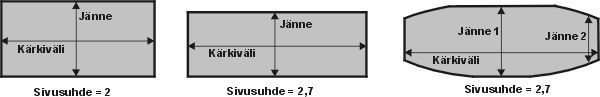
\includegraphics[width=0.9\textwidth]{Sivusuhde.jpeg}\caption{Sivusuhteeltaan ja muodoltaan erilaisia kupuja. Vasemmalla on matalan sivusuhteen kupu, keskellä korkean sivusuhteen neliskanttinen kupu ja oikealla korkean sivusuhteen elliptinen kupu. Kupujen pinta-alat ovat samat.}\end{figure*} 


Seuraavalla sivulla olevassa kuvassa on erimuotoisia kupuja, jotka ovat samankokoisia, mutta joiden sivusuhteet ovat erilaiset. Vasemmalla olevan kuvun sivusuhde on pienempi (low aspect ratio) kuin kahden muun, koska kuvun kärkivälin suhde jänteeseen on pienempi. Sivusuhde vaikuttaa kuvun aerodynamiikkaan siten, että suuremmalla sivusuhteella varustettu kupu (siis hoikempi) tuottaa enemmän nostetta suhteessa vastukseen. Teoriassa isomman sivusuhteen kupu lentää nopeammin, paremmalla liitosuhteella ja on tehokkaampi fleerissä kuin pienemmän sivusuhteen kupu. Tässä havaitaan ensimmäinen oleellinen ero 9-tunnelisten ja 7-tunnelisten varjojen välillä: 9-tunnelisella varjolla on suurempi sivusuhde kuin 7-tunnelisella, joten niiden liitosuhde on yleensä myös parempi. Mitä suurempi sivusuhde kuvussa on, sitä vaikeampi reunimmaisia tunneleita on saada pysymään paineistettuna ja täten saada siipi pysymään muodossaan. Tätä voidaan auttaa lisäämällä tunneleiden lukumäärää, jolloin myös kuvun rakenne muuttuu kiinteämmäksi. Käytännössä tämänhetkisten varjojen sivusuhteet ovat 7-tunnelisten kohdalta noin 2,2:1 kun taas 9-tunnelisissa kuvuissa jopa lähes 3:1. 


Miksi ei sitten rakenneta vaikkapa 11-tunnelista varjoa hyvin suurella sivusuhteella? Jokainen tunneli lisää väliseiniä kuvun sisälle ja tarvitsee kantopunokset pysyäkseen muodossaan. Lisätyt punokset sekä saumat vahvikenauhoineen varjossa lisäävät varjon ilmanvastusta, kasvattavat sen pakkaustilavuutta ja nostavat samalla valmistuskustannuksia. Suuren sivusuhteen varjot (high aspect ratio) vastaavat ohjaukseen herkemmin ja vajaatoiminnot sekä sakkaus ovat radikaalimpia. Myös vajaatoiminnoista palautuminen (kuvun paineistuminen) voi olla epätasaisempaa. Lisäksi suuren sivusuhteen varjot kääntyvät nopeammin kuin samankokoiset pienen sivusuhteen varjot (itse asiassa pienen sivusuhteen varjo aloittaa käännöksen kyllä nopeammin, erityisesti syvässä jarrutustilassa, mutta itse käännösnopeus on suurempi suuren sivusuhteen varjoissa). Samoin kuin sakkauksesta palautuessa, myös avauksissa pienemmän sivusuhteen varjoilla on tasaisemmat täyttymisominaisuudet. Tästä syystä kaikki kupumuodostelmahyppäämiseen tarkoitetut päävarjot ja lähes kaikki varavarjot ovat pienen sivusuhteen 7-tunnelisia varjoja. 


Kumpi sitten on parempi, 9-tunnelinen (suurempi sivusuhde) vai 7-tunnelinen (pienempi sivusuhde)? Molemmissa on puolensa, kuten jo aiemmin todettiin. 9-tunnelisessa varjossa on enemmän nostetta kuin 7-tunnelisessa. Kolikon kääntöpuolella on kuitenkin 9-tunnelisen varjon suurempi punosten ja saumojen määrä, mikä taas lisää varjon ilmanvastusta ja kuvun epätasaisuutta (joka taas kasvattaa vastusta). Käytännössä 7-tunnelisilla varjoilla on hieman jyrkempi liitokulma kuin 9-tunnelisilla, ja niillä voidaan usein laskeutua paremmin hitailla nopeuksilla. Tästä johtuen esimerkiksi tarkkuusvarjot ovat 7-tunnelisia. 7-tunnelinen varjo on myös vakaampi turbulenteissa olosuhteissa, koska paineistus reunatunneleissa on parempi. 

\section{ Elliptisyys }
\label{varjon-ominaisuudet-elliptisyys}


Elliptisellä varjolla tarkoitetaan sellaista varjoa, jossa kaikki tunnelit eivät ole samanpituisia, eli kuvun jänne ei ole vakio kaikista kohdista mitattuna. Elliptisen kuvun reunatunnelit ovat keskitunneleita lyhyempiä ja joskus myös kapeampia. Puhuttaessa täyselliptisestä varjosta tarkoitetaan sellaista varjoa, jossa sekä etu- että takahelma ovat kaarevia. \textit{Semielliptisellä} kuvulla tarkoitetaan kupua, jossa vain takahelma on kaareva. Näitä varjoja valmistettiin muutama vuosi sitten etenkin kohderyhmänä tuoreet kelpoisuushyppääjät. Semielliptisyys on jossakin määrin vanhentunut käsite, sillä nykyään valmistetaan paljon täyselliptisiä varjoja, jotka on kuitenkin suunniteltu kokemattomillekin hyppääjille ja täten puhutaan vain kokemattomille hyppääjille soveltuvista varjoista. Tällaisia varjoja kutsutaan esim. \textit{tapered} varjoiksi erotuksena voimakkaasti elliptisistä varjoista. Tätä opasta kirjoitettaessa suurin osa valmistettavista kuvuista on ei-suorakaiteen muotoisia; jopa oppilaat hyppäävät (joskin lievästi) elliptisillä varjoilla. 


Elliptisen siiven ehkä tärkein perusominaisuus on se, että siiven elliptisen muodon takia sen siivenkärki (kuvun reuna) on lyhyempi kuin siiven jänne siiven keskiosassa. Kuvun lentäessä ilman läpi siivenkärki aiheuttaa kärkipyörteen, joka aiheuttaa siipeä jarruttavaa indusoitua vastusta. Kärkipyörrettä voidaan vähentää tekemällä suuren sivusuhteen kupu, jossa siivenkärki suhteessa kuvun kokoon on pienempi. Elliptisellä muodolla saadaan siivenkärki yhä pienemmäksi ja edelleen vähennettyä kärkipyörteen (ja siten myös indusoidun vastuksen) syntymistä. Indusoidun vastuksen vähenemisen on osatekijä sille, että elliptinen kupu tuottaa enemmän nostetta, on herkempi ohjattava ja fleeraa paremmin. Tähän vaikuttaa myös elliptisen kuvun parempi paineistus. 


Laskuvarjoa suunniteltaessa tärkeä suunnitteluparametri on myös nosteen keskipiste (center of lift). Jos varjo suunnitellaan siten, että nosteen keskipiste on lähellä kuvun etureunaa, varjolla on hyvin jyrkkä liitokulma ja kuvun paineistus on hyvin stabiili. Siirrettäessä nosteen keskipistettä taemmas, lähemmäs jänteen keskipistettä, varjon liitokulma pienenee (paranee), mutta samalla kuvun paineistus muuttuu epästabiilimmaksi. Samalla, jos kuvulla on suuri siipisuhde, sen reunatunnelit tai niiden kulmat saattavat tukahtua käännösten aikana, koska tunneleissa ei enää riitä painetta pitämään niitä muodossa. Elliptiset kuvut ratkaisevat myös tätä ongelmaa, sillä kun reunatunnelit ovat keskitunneleita lyhyempiä, pysyvät ne myös paremmin paineistettuina. Elliptiset varjot reagoivat yleensä ohjausliikkeisiin helpommin ja ovat herkempiä ohjattavia kuin ei-elliptiset. 

\section{ Kuvun siipiprofiili }
\label{varjon-ominaisuudet-kuvun-siipiprofiili}


Kuvun profiililla (tai siipiprofiililla) tarkoitetaan kuvun sivuprofiilia. Kuvun profiili määrää suuren osan varjon ominaisuuksista. Tyypillisesti 7-tunneliset varjot ovat \textit{korkeaprofiilisia}, eli kuvun tunnelit ovat korkeampia ja niiden suuaukot isompia kuin 9-tunnelisissa matalaprofiilisissa varjoissa. Kuvun korkeampi profiili lisää vastusta mutta toisaalta tuottaa enemmän nostetta hitaalla ilmanopeudella. Korkeaprofiilisilla varjoilla on yleensä paremmat ominaisuudet lennettäessä hitaasti ja kovilla jarruilla. Myös tästä syystä tarkkuusvarjot ovat korkeaprofiilisia 7-tunnelisia varjoja. Myös varjon muita ominaisuuksia, kuten liitokulmaa, voidaan säädellä profiilin muotoilulla, ja kupujen profiilit ovatkin kehittyneet varjojen kehityksen myötä aina tarkemmiksi ja tehokkaammiksi. Uudemmissa varjoissa olevat aerodynaamisesti tehokkaammat ja matalammat siipiprofiilit kykenevät tuottamaan enemmän nostetta suhteessa vastukseen, ja niinpä tehokkaampiprofiilisella varjolla voidaan lentää suuremmalla siipikuormalla silti heikentämättä laskeutumisominaisuuksia. Varjojen profiilien kehityksestä johtuu osaltaan se, että vanhoilla varjoilla ei usein voida (ei kannata) lentää suurilla (>1,5) siipikuormilla, kun taas nykyaikaisille varjoille kyseiset kuormat ovat arkipäivää. 

\section{ Muut varjojen rakenteelliset ominaisuudet }
\label{varjon-ominaisuudet-muut-varjojen-rakenteelliset-ominaisuudet}


Nykyaikaisissa laskuvarjoissa on myös eräitä niiden suorituskykyyn ja käyttäytymiseen vaikuttavia rakenteellisia lisäratkaisuja, jotka lyhyesti esitellään tässä kappaleessa. Useimmiten käytössä olevien kupujen rakenne on sellainen, että tunneli on itse asiassa tunnelipari (9-tunnelisessa kuvussa on siis 18 tunnelia). Nykyään valmistetaan kokeneille hyppääjille ja kilpailukäyttöön erittäin suorituskykyisiä varjoja, joissa kuvun kukin tunneli jakaantuu kolmeen osaan. Tällaista kuvun rakennetta kutsutaan tri-cell-rakenteeksi. Tällöin siis esimerkiksi 7-tunnelisessa tri-cell-kuvussa onkin itse asiassa 21 ja 9-tunnelisessa 27 tunnelia. Tri-cell-rakenteen etu on pienempi tunnelikoko ja suurempi kupua tukevien rakenteiden määrä. Näin kuvusta saadaan kiinteämpi, ja sen siipiprofiilia voidaan tehdä ohuemmaksi. Pienempi kupu ja ohuempi siipiprofiili vähentävät myös kuvun aiheuttamaa ilmanvastusta ja parantavat kuvun aerodynaamisia ominaisuuksia. Kun kupu on kiinteämpi ja aerodynaamisesti tehokkaampi, sillä voidaan lentää suuremmalla siipikuormalla, mikä myös parantaa kuvun paineistusta. Tri-cell-varjoissa käytetään yleensä kuvun tukevoittamiseen ristituentaa (crossbracing). Ristituennalla tarkoitetaan tri-cell-kuvun tunnelikolmikon reunimmaisiin tunneleihin sijoitettuja tunnelissa poikittain kulkevia tukia. Ristitukien avulla siipi saadaan entistäkin kiinteämmäksi, ja kupu pysyy paremmin muodossaan fleerin aikana, jolloin kuvun tehokas pinta-ala pysyy mahdollisimman suurena. Tämä lisää fleerin tehoa ja mahdollistaa myös suuremman siipikuorman (pienemmän kuvun) käytön. Huonona puolena ovat suuremmat valmistuskustannukset monimutkaisen rakenteen takia sekä suurempi pakkaustilavuus. Ristituettuja tri-cell-varjoja ovat esimerkiksi PD Velocity, Icarus Extreme VX/FX sekä Precision Aerodynamics Xaos 21/27. 


\begin{Figure}\centering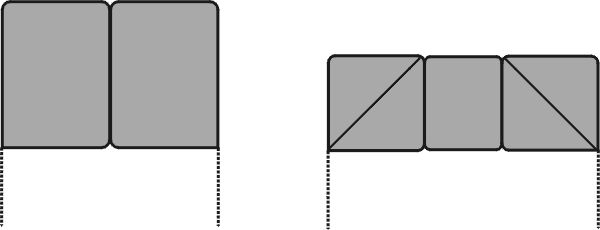
\includegraphics[width=0.7\textwidth]{Tunneli-perinteinen-xbrace.jpeg}\captionof{figure}{Perinteinen tunnelipari ja ristituettu tri-cell -tunnelikolmikko.}\end{Figure} 


Ilmalukoilla (airlocks) pyritään myös vaikuttamaan kuvun tukevuuteen. Ilmalukot ovat kuvun etureunassa tunneliaukkojen suulla oleva kankainen venttiilirakenne, joka mahdollistaa ilman pääsemisen kuvun sisään (eli kuvun paineistumisen), mutta vaikeuttaa ilman pääsemistä kuvusta ulos, jolloin kupu pysyy paremmin paineistettuna. Ilmalukot auttavat kuvun pysymistä paineistettuna esim. erittäin turbulenttisissa olosuhteissa. Ilmalukolliset kuvut säilyttävät muotonsa paremmin myös fleerin loppuvaiheessa. Huonona puolena ovat suuremmat valmistuskustannukset ja suurempi pakkaustilavuus. Ilmalukollisia kupuja valmistaa lähinnä USA:lainen Big Air Sportz (Lotus, Samurai, Sensei). 

\section{ Muut laskuvarjon aerodynamiikkaan vaikuttavat tekijät }
\label{varjon-ominaisuudet-muut-laskuvarjon-aerodynamiikkaan-vaikuttavat-tekijat}


Edellisessä kappaleessa käsiteltiin muutamia kupujen rakenteellisia asioita ja niiden vaikutuksia kuvun ominaisuuksiin. Tässä kappaleessa käsitellään muita laskuvarjojen yleisiä teknisiä ratkaisuja ja niiden vaikutuksia laskuvarjon aerodynamiikkaan. 


Kuten edellisessä kappaleessa todettiin, suuri osa laskuvarjon vastuksesta aiheutuu rakenteellisista ratkaisuista. Kupua suunniteltaessa vastusta pyritään vähentämään esimerkiksi matalalla siipiprofiililla. Laskuvarjon ilmanvastukseen vaikuttavat myös muut järjestelmän osat, kuten esimerkiksi valjaissa olevat tekniset ratkaisut ja itse hyppääjä. Useimmissa varjoissa on nykyään ilmanvastusta vähentävä \textbf{tukahdutettava slider} (kill-line slider) sekä \textbf{tukahtuva apuvarjo}. Slider voidaan tukahduttaa kill-lineilla avauksen jälkeen ja vetää alas kantohihnojen alapäähän, jolloin sliderin kangasta on mahdollisimman vähän ilmavirrassa lisäämässä ilmanvastusta. Lisäksi tukahduttaminen vähentää sliderin hakkaamista punoksia vasten. Ilmavirran aiheuttama hakkaaminen kuluttaa punoksia.  


Apuvarjo tukahtuu avauksen jälkeen automaattisesti. Apuvarjon tukahtumisella vähennetään sen aiheuttamaa vastusta ja saadaan näin kupu pysymään paremmin muodossa, kun apuvarjo ei aiheuta vetoa yhdyspunoksen kiinnityskohtaan. Molempia edellä mainittuja ratkaisuja käytetään nykyisin lähes kaikissa lisenssihyppääjien käyttämissä varusteissa. 


Sliderin vetäminen alas parantaa kuvun aerodynaamisia ominaisuuksia myös antamalla kantohihnojen levitä vapaammin sivuille. Tällöin kuvun muoto paranee, ja se lentää litteämpänä kehittäen enemmän nostetta. Kantohihnojen leviämistä sivuille ja siten kuvun avautumista leveämmäksi voidaan myös helpottaa löysäämällä rintahihna avauksen jälkeen. Rintahihnan löysäämisellä ei kuitenkaan ole vaikutusta kuvun aerodynaamisiin ominaisuuksiin vasta kuin hyvin suurilla siipikuormilla lennettäessä ja hyvin suorituskykyisestä varjosta optimaalista suorituskykyä haettaessa. Rintahihnan löysääminen tuo mukanaan huomattavia riskejä, mikäli joudutaan varavarjon käyttöä vaativaan vajaatoimintaan myöhemmässä vaiheessa hyppyä, joten rintahihnan löysääminen ei ole suositeltavaa.  


Kuvun leviämistä voidaan auttaa myös \textbf{kolmansilla viilekkeillä} (triple risers). Kolmannet viilekkeet ovat takimmaisiin kantohihnoihin kiinnitettävät erilliset lisäkantohihnat, joiden päässä olevan ohjurirenkaan läpi ohjauspunos kulkee. Tällöin ohjauspunokset pääsevät kulkemaan enemmän sivuilta ja varjon takahelma pääsee levittymään enemmän. Kolmannet viilekkeet ovat joidenkin suosiossa, mutta kiistatonta näyttöä niiden suorituskykyä lisäävistä ominaisuuksista ei ole. Kolmannet viilekkeet mahdollistavat käsien sivuttaisliikkeen käytön tasapainon hallintaan esim. laudan kanssa laskeuduttaessa, ja jotkut skysurf-hyppääjät käyttävätkin niitä sen vuoksi. Kolmansien viilekkeiden käyttö on viime vuosina vähentynyt merkittävästi ja nykyaikaisessa kalustossa niitä näkee enää harvoin. 


Kilpailukäyttöön sekä tehtaiden testihyppääjille on olemassa irrotettavia avausjärjestelmiä, joita käytettäessä avausjärjestelmän (apuvarjo, yhdyspunos sekä slider) aiheuttama vastus poistuu kokonaan. Näiden järjestelmien yleistymistä hidastavat niiden käytön hankaluus sekä mukanaan tuoma lisävaiva. Lisäksi järjestelmien tuoma hyöty tulee ilmi vasta, kun varjosta osataan käyttää lähes 100 \% sen suorituskyvystä. 


Suuren osan laskuvarjon vastuksesta aiheuttavat punokset. Punosten aiheuttamaa vastusta pyritään vähentämään kehittämällä yhä ohuempia ja samalla pienempivastuksisia punosmateriaaleja. Seuraavassa esitellään lyhyesti tällä hetkellä käytössä olevat yleisimmät punosmateriaalit sekä niiden ominaisuudet: 

\begin{itemize}
\item  \textbf{Dacron}: Paksu ja kulutuskestävä punosmateriaali; yleisesti käytössä oppilas- sekä tandemvarjoissa. 
\item  \textbf{Spectra}: Yleisin punosmateriaali, (myös nimellä \textit{Microline}) on kohtalaisen ohutta ja kulutusta kestävää materiaalia. Huono puoli on kutistuminen sliderin aiheuttaman kitkalämmön vuoksi.  
\item  \textbf{Vectran}: Ei kutistu ja on halkaisijaltaan hieman ohuempaa kuin Spectra. Huono puoli on Spectraa heikompi kulutuskestävyys ja se, että kuluminen ei näy niin selkeästi kuin Spectrassa. 
\item  \textbf{HMA}: Lyhenne sanoista High Modulus Aramide. On käytössä tietyissä erittäin suorituskykyisissä kupumalleissa. HMA-punos on halkaisijaltaan erittäin ohutta. Huono puoli on heikko kulutuskestävyys.  
\end{itemize}

Punosten vaikutusta varjon aerodynamiikkaan ei pidä vähätellä, sillä paljon hypätty punossetti on usein syynä varjon ominaisuuksien heikkenemiseen. Kutistuminen tapahtuu pikkuhiljaa ja jää usein havaitsematta, koska hyppääjä tottuu kupunsa muuttuviin ominaisuuksiin niiden tapahtuessa vähitellen. Kuvun punokset kutistuvat voimakkaammin reunoilta sliderin hangatessa reunimmaisia punoksia eniten. Punossetti tulisikin vaihtaa riittävän usein. 

